\documentclass[10pt,letterpaper]{article}
\usepackage[table]{xcolor}
\usepackage{tabularx}
\usepackage{booktabs}
\usepackage{float}
\usepackage{array}

% Carga la configuración global
\usepackage[utf8]{inputenc}
\usepackage[spanish]{babel}
\usepackage[margin=1.5cm]{geometry}
\usepackage{xcolor}
\usepackage{tabularx}
\usepackage{booktabs}
\usepackage[table]{xcolor}
\usepackage{enumitem}
\usepackage{hyperref}
\usepackage{fancyhdr}
\usepackage{amsmath}
\usepackage{amssymb} % Paquete requerido para \blacksquare
\usepackage{graphicx}
% Colores institucionales UNAL y formato de tablas
\definecolor{unalnavy}{HTML}{003366}
\definecolor{unalblue}{HTML}{4682B4}
\definecolor{rowalt}{HTML}{F4F7F9}
\definecolor{categorybg}{HTML}{D9E1E8}
\definecolor{bordergrey}{HTML}{B0B0B0}

\setlength{\arrayrulewidth}{0.8pt}

% Encabezado y pie de página
\pagestyle{fancy}
\fancyhf{}
\rhead{\color{unalnavy}\bfseries DR-VF-01 | Cerca Virtual}
\lhead{\color{unalnavy}\bfseries UNAL - DIEEC}
\rfoot{\small Página \thepage}
\lfoot{\small Septiembre 2026 | Rev. 1.0}
\renewcommand{\headrulewidth}{0.8pt}
\renewcommand{\footrulewidth}{0.4pt}

\usepackage{tikz}
\usetikzlibrary{arrows.meta, positioning, shapes.geometric}

\begin{document}

% Encabezado institucional del proyecto
\begin{center}
    {\Huge \bfseries UNAL}\\[0.15cm]
    {\Large \bfseries DR-VF-01 | PRODUCT AND SYSTEM REQUIREMENTS}\\[0.1cm]
    {\large \bfseries Collar Inteligente para Cerca Virtual y Monitoreo Ganadero}\\[0.1cm]
    {\small \color{gray} Departamento de Ingeniería Eléctrica, Electrónica y Computación (DIEEC) -- Sede Manizales}\\
    {\small \color{gray} Asignatura: Proyecto de Ingeniería Electrónica | \url{https://fia.unal.edu.co}}
\end{center}

\vspace{-0.2cm}
\hrule height 1pt
\vspace{0.3cm}

% --- MÓDULOS DE CONTENIDO ---
\section*{Descripción del problema de diseño}
En la gestión ganadera extensiva, el control del perímetro mediante cercados físicos tradicionales representa un elevado costo de instalación, mantenimiento constante por caídas de árboles o animales, e inflexibilidad para implementar sistemas de pastoreo rotacional eficiente. El problema de diseño consiste en definir y documentar la arquitectura de grado industrial de un \textbf{Collar Inteligente de Cerca Virtual y Monitoreo en Tiempo Real (DR-VF-01)}, capaz de delimitar potreros dinámicos mediante geolocalización satelital multiconstelación a alta frecuencia y emitir estímulos disuasivos progresivos (sonoros y electrostáticos aislados de $0.2~\text{J}$ bajo la norma IEC 60335-2-76) cuando el bovino intenta sobrepasar los límites permitidos.

\begin{itemize}[leftmargin=*, label=$\blacksquare$]
    \item \textbf{Autonomía y Balance Energético MPPT:} Integración de un sistema de recarga conmutado por punto de máxima potencia (MPPT CN3791) y batería de tecnología LiFePO4 de alta estabilidad térmica ($60\,^\circ\text{C}$), alimentando el módem IoT LTE Cat-M1/NB-IoT en modo PSM ($3.9~\mu\text{A}$) y el receptor GNSS multiconstelación.
    \item \textbf{Procesamiento en el Borde e Inteligencia Artificial (Edge AI):} Ejecución local en el microcontrolador de alto rendimiento (ESP32-S3-N16R8) de algoritmos geométricos (\textit{Point-in-Polygon} a $10~\text{Hz}$) y clasificación inercial de la conducta del animal (rumia y pastoreo) mediante el núcleo de Machine Learning integrado en la IMU ST LSM6DSOX.
    \item \textbf{Seguridad, Aislamiento y Resiliencia Hardware:} Aislamiento de $5~\text{kV}_{\text{RMS}}$ entre la lógica de control ($3.3~\text{V}$) y la etapa de alto voltaje disuasivo ($2.5~\text{kV}$ / $0.2~\text{J}$), complementado con un temporizador \textit{Watchdog} externo dedicado (TPS3823) para prevenir bloqueos por interferencia electromagnética.
    \item \textbf{Resistencia Mecánica y Estanqueidad IP68:} Encapsulado industrial en policarbonato PC+ABS resistente a radiación UV con membrana de descompresión Gore Vent, capaz de soportar impactos, sumersión en barro y variaciones térmicas extremas.
    \item \textbf{Costo Target de Grado Comercial:} Mantener el costo total de la lista de materiales (\textit{Target BOM}) optimizado en \textbf{\$56.80~USD ($\sim$\$227.000~COP)} por unidad, garantizando viabilidad comercial para producción en serie.
\end{itemize}

\section*{Descripción técnica del sistema}
La arquitectura funcional de grado industrial del collar se organiza en los siguientes bloques principales:

\begin{enumerate}[leftmargin=*]
    \item \textbf{Etapa de Cosecha Solar y Gestión de Potencia:} Panel solar monocristalino (5~V / 1.5~W), controlador de carga MPPT (CN3791), circuito de protección de celda (BQ2970), medidor de carga por conteo de Coulomb ($\text{I}^2\text{C}$ MAX17048) y batería industrial LiFePO4 de 3.2~V (3200~mAh, $>2000$ ciclos útiles).
    \item \textbf{Unidad de Procesamiento Central (MCU):} Microcontrolador ESP32-S3 Dual-Core (16~MB Flash, 8~MB PSRAM) a cargo del cálculo de geocercas en tiempo real, gestión de actualización remota de firmware (\textit{Dual-Bank OTA}), servidor web local (LittleFS) y punto de acceso Wi-Fi/BLE para configuración offline.
    \item \textbf{Subsistema de Posicionamiento Satelital GNSS:} Receptor multiconstelación de alta precisión u-blox MAX-M10S (GPS, GLONASS, Galileo, Beidou) operando a una frecuencia de muestreo adaptativa de hasta 10~Hz mediante bus UART.
    \item \textbf{Subsistema de Telemetría Dual (Celular IoT + LoRa):} Módem celular de bajo consumo Quectel BG95-M3 (LTE Cat-M1 / NB-IoT / EGPRS) y transceptor de radiofrecuencia de larga distancia Semtech SX1262 (LoRa 915~MHz a $+22~\text{dBm}$) para zonas sin cobertura celular.
    \item \textbf{Etapa de Estimulación Disuasiva Aislada (HV Interlock):} Transistor driver con optoacoplador de alta aislación ($5~\text{kV}_{\text{RMS}}$), temporizador de corte por hardware de doble interruptor (\textit{interlock}), elevador de voltaje de ferrita limitado a $0.2~\text{J}$ ($2.5~\text{kV}$) según norma IEC 60335-2-76 y zumbador piezoeléctrico de advertencia.
    \item \textbf{Subsistema Inercial e Inteligencia de Borde (IMU + MLC):} Acelerómetro y giroscopio de 6 ejes ST LSM6DSOX con Núcleo de Machine Learning (MLC) integrado para la detección pasiva de patrones de salud, caminata y rumia.
    \item \textbf{Memoria No Volátil de Alta Durabilidad y Supervisión:} Memoria ferroeléctrica FRAM SPI (MB85RS64V, $10^{14}$ ciclos) para retención instantánea de polígonos/estados de la FSM y \textit{Watchdog} hardware externo independiente (TPS3823) conectado al pin de reinicio principal.
\end{enumerate}
\section*{Casos de Uso -- Collar Inteligente para Cerca Virtual (Arquitectura V4.1)}

\begin{table}[H]
    \centering
    \small
    \renewcommand{\arraystretch}{1.3}
    \rowcolors{2}{white}{gray!8}
    \begin{tabularx}{\linewidth}{|c|X|X|}
        \hline
        \rowcolor{gray!20}
        \textbf{Caso} & \textbf{Descripción} & \textbf{Requerimientos Derivados (Hardware V4.1)} \\ \hline
        1 & Monitoreo estándar dentro de zona segura: El animal se desplaza libremente en el polígono. & GNSS u-blox MAX-M10S en muestreo adaptativo, módem Quectel BG95-M3 en modo PSM ($3.9~\mu\text{A}$) y transmisión periódica LTE Cat-M1/NB-IoT. \\ \hline
        2 & Aproximación a zona de advertencia ($3\text{ a }5~\text{m}$ del borde): IMU/GNSS detecta trayectoria hacia el límite. & Incremento dinámico del GNSS a $10~\text{Hz}$ y activación inmediata del zumbador piezoeléctrico como estímulo sonoro preventivo. \\ \hline
        3 & Traspaso del límite (Infracción de geocerca): El bovino ignora el sonido y cruza el perímetro. & Activación del pulso disuasivo aislado ($0.2~\text{J}$ a $2.5~\text{kV}$, IEC 60335-2-76) mediante optoacoplador VO617A e \textit{interlock} hardware; envío de alerta prioritaria. \\ \hline
        4 & Configuración de potrero offline por el ganadero: El usuario define un nuevo lote en campo sin red. & ESP32-S3 genera punto de acceso Wi-Fi SoftAP / BLE, sirve la web app desde LittleFS y guarda las coordenadas en la memoria FRAM (MB85RS64V). \\ \hline
        5 & Operación en zona rural sin cobertura celular: Finca remota sin señal LTE/EGPRS. & Conmutación automática a telemetría de largo alcance mediante transceptor LoRa Semtech SX1262 ($+22~\text{dBm}$) hacia Gateway local. \\ \hline
        6 & Mantenimiento energético solar continuo: Exposición a radiación solar durante pastoreo. & Algoritmo de seguimiento MPPT (CN3791) optimizando la recarga de la celda LiFePO4 de $3.2~\text{V}$ ($3200~\text{mAh}$, tolerante hasta $60\,^\circ\text{C}$). \\ \hline
        7 & Ahorro de energía por inactividad/rumia: El animal descansa o rumia en el potrero. & El Núcleo de Machine Learning (MLC) de la IMU ST LSM6DSOX clasifica la conducta; ESP32-S3 entra en \textit{Deep Sleep} ($7~\mu\text{A}$) con \textit{Watchdog} TPS3823 activo. \\ \hline
        8 & Carga previa / Diagnóstico por cable: Mantenimiento o configuración rápida en establo. & Puerto USB-C nativo del ESP32-S3, CI de protección BQ2970 y calibración de estado de carga (SoC) mediante el medidor MAX17048. \\ \hline
        9 & Degradación de señal GNSS por follaje denso: Pérdida o atenuación satelital en dosel forestal. & Operación multiconstelación (GPS, GLONASS, Galileo, Beidou) con filtro LNA/SAW, filtrado de Kalman y almacenamiento offline en Flash (16~MB). \\ \hline
        10 & Alerta de carga crítica de batería: Disminución de capacidad tras días nublados continuos. & El medidor de Coulomb MAX17048 por $\text{I}^2\text{C}$ detecta SoC $\le 10\%$ (superando la curva plana de LiFePO4), envía alerta SMS/MQTT y conmuta a modo supervivencia. \\ \hline
    \end{tabularx}
\end{table}
\section*{Requerimientos del Producto (PRD)}

\begin{table}[H]
    \centering
    \small
    \renewcommand{\arraystretch}{1.3}
    \rowcolors{2}{white}{gray!8}
    \begin{tabularx}{\linewidth}{|c|X|c|}
        \hline
        \rowcolor{gray!20}
        \textbf{ID} & \textbf{Descripción del requerimiento} & \textbf{Tipo} \\ \hline
        F-01 & El sistema debe determinar la ubicación geográfica mediante GPS con actualización $\ge 1~\text{Hz}$. & Funcional \\ \hline
        F-02 & El microcontrolador debe ejecutar algoritmos Haversine y Point-in-Polygon en tiempo real. & Funcional \\ \hline
        F-03 & El dispositivo debe contar con disuasión en dos etapas: alerta acústica y pulso electrostático. & Funcional \\ \hline
        F-04 & El sistema debe contar con aislamiento galvánico mediante optoacoplador (PC817). & Funcional \\ \hline
        F-05 & El collar debe integrar conectividad dual: GSM/2G para SMS/GPRS y LoRa para red privada. & Funcional \\ \hline
        F-06 & Configuración de geocerca mediante servidor web interno accesible por Wi-Fi. & Funcional \\ \hline
        F-07 & Carga híbrida: entrada fotovoltaica (Panel 5~V) y entrada USB-C (5~$\text{V}_{\text{DC}}$). & Funcional \\ \hline
        F-08 & Corte de alimentación independiente mediante MOSFETs para apagar GPS/GSM en reposo. & Funcional \\ \hline
        NF-01 & Autonomía mínima de 15~días continuos en ausencia total de radiación solar. & No funcional \\ \hline
        NF-02 & Aislamiento galvánico con tensión de ruptura $\ge 1000~\text{V}_{\text{AC}}$ entre primario y secundario. & No funcional \\ \hline
        NF-03 & Encapsulado mecánico estanco con grado de protección equivalente a IP67. & No funcional \\ \hline
        NF-04 & Costo total de componentes (BOM) $\le \$150.000~\text{COP}$ ($\sim 35~\text{USD}$) por unidad. & No funcional \\ \hline
        NF-05 & Rango térmico de operación expuesto en campo de $-10~^\circ\text{C}$ a $50~^\circ\text{C}$. & No funcional \\ \hline
        NF-06 & Peso total del dispositivo, correa y contrapesos $\le 600~\text{g}$. & No funcional \\ \hline
        NF-07 & Coordenadas del perímetro guardadas en memoria no volátil (NVS). & No funcional \\ \hline
        NF-08 & PCB diseñada a 2 capas en Altium Designer para fácil manufactura. & No funcional \\ \hline
    \end{tabularx}
\end{table}
\section*{Requerimientos del Sistema (SRD)}

\begin{table}[H]
    \centering
    \small
    \renewcommand{\arraystretch}{1.3}
    \rowcolors{2}{white}{gray!8}
    \begin{tabularx}{\linewidth}{|c|X|X|X|}
        \hline
        \rowcolor{gray!20}
        \textbf{ID} & \textbf{Descripción} & \textbf{Especificación / Valor} & \textbf{Verificación} \\ \hline

        \multicolumn{4}{|l|}{\cellcolor{gray!20}\textbf{Entrada y Gestión de Energía}} \\ \hline
        \textbf{SR-01} & Cosecha de energía solar & Panel monocristalino $5\text{ V DC}$, $1.5\text{ W} \text{--} 2.0\text{ W}$ & Prueba funcional con fuente DC / simulador \\ \hline
        \textbf{SR-02} & Carga externa cableada & Puerto USB-C ($5\text{ V DC} \pm 5\%$, CI TP4056/CN3065) & Medición de perfil de carga CC/CV \\ \hline
        \textbf{SR-03} & Almacenamiento de energía & Batería LiPo 3.7 V / 2500 mAh con PCM de protección & Ensayo de descarga a tasa $0.2\text{C}$ \\ \hline
        \textbf{SR-04} & Consumo en ultra bajo consumo & $\le 15\,\mu\text{A}$ en modo Deep Sleep (corte por MOSFETs) & Medición con microamperímetro \\ \hline
        \textbf{SR-05} & Autonomía sin radiación & $\ge 15\text{ días}$ continuos sin radiación solar & Ensayo de consumo acumulado en cámara \\ \hline

        \multicolumn{4}{|l|}{\cellcolor{gray!20}\textbf{Posicionamiento Satelital y Edge Computing}} \\ \hline
        \textbf{SR-10} & Frecuencia de refresco GPS & $\ge 1\text{ Hz}$ en modo activo (tramas NMEA GGA/RMC) & Analizador lógico sobre bus UART \\ \hline
        \textbf{SR-11} & Precisión de geolocalización & $\le 2.5\text{ m}$ CEP en campo abierto & Comparación contra punto geodésico \\ \hline
        \textbf{SR-12} & Tiempo de cálculo de geocerca & Latencia $\le 50\text{ ms}$ (Haversine + Point-in-Polygon) & Profiling de código en microcontrolador \\ \hline
        \textbf{SR-13} & Retención de perímetro & Coordenadas guardadas en memoria Flash NVS no volátil & Prueba de ciclo de apagado total \\ \hline

        \multicolumn{4}{|l|}{\cellcolor{gray!20}\textbf{Telemetría y Comunicaciones Duales}} \\ \hline
        \textbf{SR-20} & Transmisión Cellular (GSM/2G) & Módulo SIM800L (Soporte ráfagas de corriente $\le 2\text{ A}$) & Osciloscopio sobre riel de $3.8\text{ V}$ \\ \hline
        \textbf{SR-21} & Enlace de radio de largo alcance & Módulo LoRa SX1278 ($915\text{ MHz}$, alcance $\ge 2\text{ km}$ LoS) & Medición de RSSI/SNR y tasa PER \\ \hline
        \textbf{SR-22} & Interfaz de configuración local & Servidor Web HTTP embebido vía Wi-Fi AP ($2.4\text{ GHz}$) & Validación de carga desde navegador móvil \\ \hline

        \multicolumn{4}{|l|}{\cellcolor{gray!20}\textbf{Actuación, Disuasión y Seguridad}} \\ \hline
        \textbf{SR-30} & Estímulo sonoro preventivo & Buzzer piezoeléctrico $\ge 85\text{ dBA @ 1 m}$ ($3\text{--}5\text{ m}$ previa valla) & Sonómetro calibrado a $1\text{ m}$ \\ \hline
        \textbf{SR-31} & Estímulo electrostático disuasivo & Pulso de alto voltaje / muy baja corriente al cruzar valla & Medición de energía con sonda HV \\ \hline
        \textbf{SR-32} & Aislamiento galvánico & Optoacoplador PC817 (Ruptura $\ge 1000\text{ VAC}$ entre fases) & Ensayo Hipot / Dielectric Withstand \\ \hline
        \textbf{SR-33} & Control de desconexión lógica & MOSFET canal P para aislamiento total de etapa HV & Inspección de señal PWM de control \\ \hline

        \multicolumn{4}{|l|}{\cellcolor{gray!20}\textbf{Ambientales, Mecánicos y Robustez}} \\ \hline
        \textbf{SR-40} & Protección contra el entorno & Estanqueidad equivalente a IP67 (Sumersión $1\text{ m}$ / $30\text{ min}$) & Prueba de inmersión en tanque \\ \hline
        \textbf{SR-41} & Rango térmico de operación & $-10\,^\circ\text{C}$ a $50\,^\circ\text{C}$ con exposición a radiación UV & Ensayos en cámara climática \\ \hline
        \textbf{SR-42} & Masa total del dispositivo & $\le 600\text{ g}$ (Incluye chasis, collar y batería) & Pesaje en balanza analítica \\ \hline

        \multicolumn{4}{|l|}{\cellcolor{gray!20}\textbf{Restricciones de Diseño y Costos}} \\ \hline
        \textbf{SR-50} & Costo target de producción (BOM) & $\le \$150.000\text{ COP} \,\, (\sim 35\text{ USD})$ por unidad armada & Cotización auditada de componentes \\ \hline
        \textbf{SR-51} & Manufacturabilidad de la PCB & Tarjeta de 2 capas en Altium Designer (Pistas $\ge 2\text{ A}$) & Revisión de reglas de diseño (DRC) \\ \hline
    \end{tabularx}
\end{table}
\section*{Priorización de requerimientos (MoSCoW)}

\begin{table}[H]
    \centering
    \small
    \renewcommand{\arraystretch}{1.3}
    \rowcolors{2}{white}{gray!8}
    \begin{tabularx}{\linewidth}{|X|c|}
        \hline
        \rowcolor{gray!20}
        \textbf{Requerimiento / Función Clave} & \textbf{Prioridad} \\ \hline
        Geolocalización GPS, algoritmo de geocerca en ESP32 y disuasión aislada & \textbf{Must} \\ \hline
        Alimentación híbrida (Panel solar + USB-C) y cargador LiPo integrado & \textbf{Must} \\ \hline
        Conectividad dual GSM/2G y LoRa para envío de alertas & \textbf{Must} \\ \hline
        Servidor Web interno por Wi-Fi para definir polígonos de potrero & \textbf{Must} \\ \hline
        Costo total de lista de materiales (BOM) $\le \$150.000~\text{COP}$ & \textbf{Must} \\ \hline
        Modo \textit{Deep Sleep} y corte de energía por MOSFETs (consumo $< 15~\mu\text{A}$) & \textbf{Should} \\ \hline
        Chasis estanco IP67 impreso en PETG con sellado de silicona & \textbf{Should} \\ \hline
        Detección de patrones de actividad con acelerómetro LIS3DH & \textbf{Could} \\ \hline
        Integración con plataforma en la nube o app nativa Android/iOS & \textbf{Won't} \\ \hline
    \end{tabularx}
\end{table}
\newpage

\begin{figure}[htbp]
    \centering
    \makebox[\textwidth][c]{%
        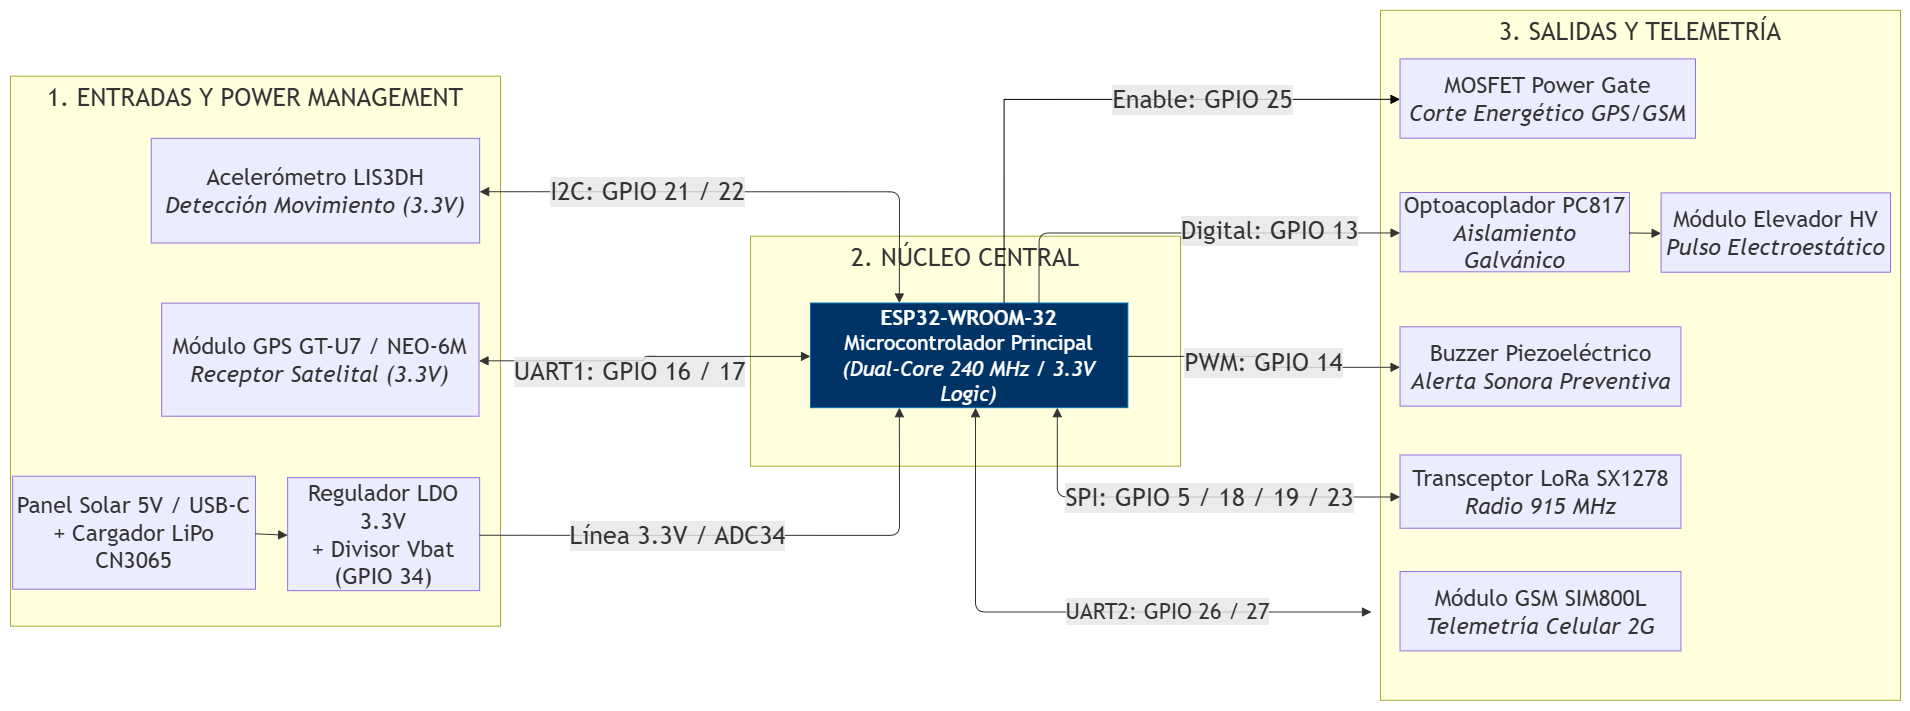
\includegraphics[width=1.1\textwidth]{Secciones/Figuras/diagrama_bloques_hardware.png}%
    }
    \vspace{0.3cm}
    \caption{Diagrama de bloques de la arquitectura de hardware del sistema DR-VF-01.}
    \label{fig:diagrama_hardware}
\end{figure}

\clearpage
%Tabla de mapeo de pines
\section*{Mapeo de Pines y Asignación de Periféricos}

\begin{table}[H]
    \centering
    \small
    \renewcommand{\arraystretch}{1.3}
    \rowcolors{2}{white}{gray!8}
    \begin{tabularx}{\linewidth}{|c|c|c|X|}
        \hline
        \rowcolor{gray!20}
        \textbf{Módulo / Periférico} & \textbf{Protocolo / Función} & \textbf{Pines ESP32} & \textbf{Notas para el Esquemático / PCB} \\ \hline
        GPS (GT-U7) & UART1 & GPIO 16 (RX), GPIO 17 (TX) & Intercambiar TX/RX en el ruteo de la PCB. \\ \hline
        GSM (SIM800L) & UART2 & GPIO 26 (RX), GPIO 27 (TX) & Requiere pista ancha de alimentación (picos de $2~\text{A}$). \\ \hline
        IMU (LIS3DH) & $\text{I}^2\text{C}$ & GPIO 21 (SDA), GPIO 22 (SCL) & Agregar resistencias pull-up de $4.7~\text{k}\Omega$ en la PCB. \\ \hline
        LoRa (SX1278) & SPI & GPIO 5 (CS), 18 (SCK), 19 (MISO), 23 (MOSI) & Mapear señal GPIO 4 para interrupción. \\ \hline
        Buzzer Piezoeléctrico & PWM & GPIO 12 & Control mediante transistor NPN o MOSFET. \\ \hline
        Optoacoplador PC817 & Digital Output & GPIO 13 & Mantener separación de planos de masa (\texttt{GND} vs. \texttt{HV\_GND}). \\ \hline
        MOSFET Power Gate & Power Control & GPIO 25 & Transistor P-Channel / N-Channel según topología. \\ \hline
        Monitoreo Batería & ADC1 & GPIO 34 & Solo entrada (\textit{Input Only}), ideal para divisor resistivo. \\ \hline
    \end{tabularx}
\end{table}


%Arbol de Potencia
\clearpage
\begin{figure}[htbp]
    \centering
    \resizebox{\linewidth}{!}{%
    \begin{tikzpicture}[
        pwr/.style={rectangle, draw=orange!80!black, fill=orange!10, thick, text width=2.4cm, text centered, rounded corners=3pt, minimum height=1.1cm, font=\sffamily\small},
        bus/.style={rectangle, draw=blue!80!black, fill=blue!10, thick, text width=2.4cm, text centered, rounded corners=3pt, minimum height=1.1cm, font=\sffamily\small},
        gate/.style={rectangle, draw=red!80!black, fill=red!10, thick, text width=2.4cm, text centered, rounded corners=3pt, minimum height=1.1cm, font=\sffamily\small},
        load/.style={rectangle, draw=gray!80, fill=gray!10, text width=2.2cm, text centered, rounded corners=3pt, minimum height=1.0cm, font=\sffamily\footnotesize},
        arrow/.style={draw, -{Latex[scale=0.9]}, thick, color=gray!70!black}
    ]

        % Capa 0: Fuentes de Entrada y Almacenamiento (y = 0)
        \node [pwr] (in) at (0,0) {Entrada 5V\\(Solar / USB-C)};
        \node [pwr] (charger) at (3.6,0) {Cargador LiPo\\(CN3065)};
        \node [pwr] (bat) at (7.2,0) {Batería LiPo\\(3.7V -- 4.2V)};

        \draw [arrow] (in) -- (charger);
        \draw [arrow] (charger) -- (bat);

        % Capa 1: Gestión y Regulación Principal (y = -2.6)
        \node [load] (gsm) at (0,-2.6) {Módulo GSM\\SIM800L\\(Picos $\le 2\text{A}$)};
        \node [bus] (ldo) at (3.6,-2.6) {Regulador LDO\\3.3V (ME6211)};
        \node [gate] (mosfet) at (7.2,-2.6) {MOSFET\\Power Gate\\(GPIO 25)};

        % Riel principal VBAT (y = -1.3)
        \draw [thick, color=gray!70!black] (bat.south) -- (7.2,-1.3);
        \node[right=3pt, font=\tiny\bfseries, color=orange!90!black] at (7.2,-0.9) {$V_{\text{BAT}}$};

        \draw [thick, color=gray!70!black] (7.2,-1.3) -- (0,-1.3);
        \draw [arrow] (0,-1.3) -- (gsm.north);
        \draw [arrow] (3.6,-1.3) -- (ldo.north);
        \draw [arrow] (7.2,-1.3) -- (mosfet.north);
        
        \node[above=2pt, font=\tiny\bfseries, color=orange!90!black] at (1.8,-1.3) {$V_{\text{BAT}}$};
        \node[above=2pt, font=\tiny\bfseries, color=orange!90!black] at (5.4,-1.3) {$V_{\text{BAT}}$};

        % Capa 2: Consumidores y Periféricos (y = -5.4)
        \node [load] (sensors) at (0,-5.4) {Sensores / Radio\\(LIS3DH / SX1278)};
        \node [load] (esp) at (2.8,-5.4) {ESP32-WROOM\\(Microcontrolador)};
        \node [load] (hv) at (5.6,-5.4) {Elevador HV\\(Pulso Eléctrico)};
        \node [load] (gps) at (8.4,-5.4) {Módulo GPS\\GT-U7};

        % Riel 3.3V (Salida LDO a y = -4.0)
        \draw [thick, color=gray!70!black] (ldo.south) -- (3.6,-4.0);
        \node[right=4pt, font=\tiny\bfseries, color=blue!80!black] at (3.6,-3.5) {3.3V};
        
        \draw [thick, color=gray!70!black] (3.6,-4.0) -- (0,-4.0);
        \draw [thick, color=gray!70!black] (3.6,-4.0) -- (2.8,-4.0);
        \draw [arrow] (0,-4.0) -- (sensors.north);
        \draw [arrow] (2.8,-4.0) -- (esp.north);

        % Riel V_SW Conmutado (Salida MOSFET a y = -4.0)
        \draw [thick, color=gray!70!black] (mosfet.south) -- (7.2,-4.0);
        \node[right=4pt, font=\tiny\bfseries, color=red!80!black] at (7.2,-3.5) {$V_{\text{SW}}$};

        \draw [thick, color=gray!70!black] (7.2,-4.0) -- (5.6,-4.0);
        \draw [thick, color=gray!70!black] (7.2,-4.0) -- (8.4,-4.0);
        \draw [arrow] (5.6,-4.0) -- (hv.north);
        \draw [arrow] (8.4,-4.0) -- (gps.north);

    \end{tikzpicture}%
    }
    \caption{Árbol de distribución de potencia y gestión energética para el sistema DR-VF-01.}
    \label{fig:arbol_potencia}
\end{figure}

%Tabla de Presupuesto Energético (Power Budget).
\section*{Presupuesto Energético y Perfil de Consumo}

\begin{table}[H]
    \centering
    \small
    \renewcommand{\arraystretch}{1.3}
    \rowcolors{2}{white}{gray!8}
    \begin{tabularx}{\linewidth}{|X|c|c|c|c|}
        \hline
        \rowcolor{gray!20}
        \textbf{Subcircuito / Módulo} & \textbf{Riel Alimentación} & \textbf{Consumo Activo} & \textbf{Consumo Reposo} & \textbf{Estado MOSFET} \\ \hline
        ESP32-WROOM & LDO $3.3~\text{V}$ & $160~\text{mA}$ & $10~\mu\text{A}$ (\textit{Deep Sleep}) & Siempre ON \\ \hline
        Sensores (LIS3DH / SX1278) & LDO $3.3~\text{V}$ & $12~\text{mA}$ & $2~\mu\text{A}$ & Siempre ON \\ \hline
        Módulo GSM (SIM800L) & Directo $V_{\text{BAT}}$ & $350~\text{mA}$ (Picos $2~\text{A}$) & $1~\text{mA}$ (\textit{Standby}) & Siempre ON \\ \hline
        Módulo GPS (GT-U7) & Conmutado $V_{\text{SW}}$ & $45~\text{mA}$ & $0~\text{mA}$ (Desconectado) & OFF en Reposo \\ \hline
        Elevador HV (Pulso) & Conmutado $V_{\text{SW}}$ & $80~\text{mA}$ (Puntual) & $0~\text{mA}$ (Desconectado) & OFF en Reposo \\ \hline
        \textbf{Consumo Total Promedio} & -- & \textbf{$\approx 647$ mA} & \textbf{$\approx 1.01$ mA} & -- \\ \hline
    \end{tabularx}
\end{table}
\section*{\color{unalnavy}Comentarios y conclusiones}

El presente documento consolida la descripción técnica de alto nivel y el conjunto de requerimientos de producto y sistema del collar inteligente para cerca virtual, concebido como una solución electrónica de bajo costo para el sector ganadero. Se establecieron las funciones esenciales que debe cumplir el dispositivo, así como las restricciones de diseño térmico, energético y de aislamiento galvánico.

Este documento no representa aún un diseño esquemático detallado ni planos de manufactura (\textit{PCB layout}), sino la línea base sobre la cual se realizarán las simulaciones, la selección final de componentes en Altium Designer y las pruebas en campo. Las limitaciones actuales comprenden la falta de pruebas de usabilidad de la interfaz web en entornos reales y la necesidad de validar el comportamiento de la batería bajo ciclos prolongados de baja radiación solar.
\section*{Revisión y Aprobación}

Este documento ha sido preparado como parte del sprint de diseño académico. La siguiente tabla garantiza el control de cambios y la validación por parte del equipo evaluador:

\begin{table}[H]
    \centering
    \small
    \renewcommand{\arraystretch}{1.3}
    \rowcolors{2}{white}{gray!8}
    \begin{tabularx}{\linewidth}{|c|X|c|c|}
        \hline
        \rowcolor{gray!20}
        \textbf{Revisión} & \textbf{Responsable} & \textbf{Fecha} & \textbf{Firma / Estado} \\ \hline
        \textbf{0.1} & Estudiantes (Equipo de diseño) & Septiembre 2026 & Borrador inicial \\ \hline
        \textbf{0.2} & Docente revisor & -- & En revisión \\ \hline
        \textbf{1.0} & Aprobado para desarrollo & -- & Pendiente \\ \hline
    \end{tabularx}
\end{table}

\end{document}